\documentclass{article}
\usepackage{arxiv}

\usepackage[utf8]{inputenc}
\usepackage[english, russian]{babel}
\usepackage[T1]{fontenc}
\usepackage{url}
\usepackage{booktabs}
\usepackage{amsfonts}
\usepackage{nicefrac}
\usepackage{microtype}
\usepackage{lipsum}
\usepackage{graphicx}
\usepackage{natbib}
\usepackage{doi}



\title{A template for the \emph{arxiv} style}

\author{ David S.~Hippocampus\thanks{Use footnote for providing further
		information about author (webpage, alternative
		address)---\emph{not} for acknowledging funding agencies.} \\
	Department of Computer Science\\
	Cranberry-Lemon University\\
	Pittsburgh, PA 15213 \\
	\texttt{hippo@cs.cranberry-lemon.edu} \\
	%% examples of more authors
	\And
	Elias D.~Striatum \\
	Department of Electrical Engineering\\
	Mount-Sheikh University\\
	Santa Narimana, Levand \\
	\texttt{stariate@ee.mount-sheikh.edu} \\
	%% \AND
	%% Coauthor \\
	%% Affiliation \\
	%% Address \\
	%% \texttt{email} \\
	%% \And
	%% Coauthor \\
	%% Affiliation \\
	%% Address \\
	%% \texttt{email} \\
	%% \And
	%% Coauthor \\
	%% Affiliation \\
	%% Address \\
	%% \texttt{email} \\
}
\date{}

\renewcommand{\shorttitle}{\textit{arXiv} Template}

%%% Add PDF metadata to help others organize their library
%%% Once the PDF is generated, you can check the metadata with
%%% $ pdfinfo template.pdf
\hypersetup{
pdftitle={A template for the arxiv style},
pdfsubject={q-bio.NC, q-bio.QM},
pdfauthor={David S.~Hippocampus, Elias D.~Striatum},
pdfkeywords={First keyword, Second keyword, More},
}

\begin{document}
\maketitle

\begin{abstract}
	\lipsum[1]
\end{abstract}


\keywords{First keyword \and Second keyword \and More}

\section{Introduction}
Let we have two distributions $\pi_0(x)$ and $\pi_1(y)$, that describes two data distributions at time 0 and time 1, respectively. Also, consider:
$$\pi_1(y) \neq \int p(y|x)\pi_0(x)dx,$$
where $p(y_1|x_0)$ -- the transition density (i.e. the probability of transitioning from $x$ at time $0$ to $y$ at time $1$) under the Brownian motion. In other words, $\pi_1(y)$ differs significantly from the distribution predicted by Brownian motion.

The Schrödinger Bridge problem considers the finding of most likely stochastic process that transforms the distribution $\pi_0(x)$ at time $0$ to $\pi_1(y)$ at time $1$ and is closer in information-theoretic sense.

So, the Schrödinger bridge provides us with a theoretically-grounded mechanism for mapping between two distribution to solve such problems like unsupervised domain adaptation and also gives the with the probability of this stochastic evolution, thus allowing us to compare two datasets/distributions which can be useful for hypothesis testing and semantic similarity

So, speaking formally, there are two approaches to problem setting, dynamic and static.

\subsection{Dynamic Schrödinger Bridge Problem}
In this approach is minimizing of KL divergence between two \textit{path measures} $\mathbb{Q}$ and $\mathbb{W}^\gamma$, path measures of our desired process and prior Wiener process with drift coefficient $\sqrt\gamma$.
$$\hat\mathbb{Q} = \arg\min_{\mathbb{Q}\in \mathcal{D}(\pi_0, \pi_1)} KL(\mathbb{Q}||\mathbb{W}^\gamma)$$

Path measure is a weak solution for given SDE, i.e. a stochastic process. Weak solution is a terminology for a solution of an SDE, that does not take into account an initial value problem and has the freedom of specifying its probability space

\subsection{Static Schrödinger Bridge Problem}
In this approach is minimizing of KL divergence between two joint distributions $q(x,y)$ and $p^{\mathbb{W}^\gamma}(x,y)$

$$\left\{ \begin{array}{c}
\hat p(x,y) = \arg\min_{q(x,y)} KL(q(x,y)||p^{\mathbb{W}^\gamma}(x,y)), \\
\pi_0(x) = \int q(x,y)dy, \\
\pi_1(y) = \int q(x,y)dx
\end{array}\right.$$
where $q(x,y)$ is a joint distribution which is closest to the Brownian-motion prior subject to marginal constraints (between PDF at time 0 and 1)
\section{Headings: first level}
\label{sec:headings}

\lipsum[4] See Section \ref{sec:headings}.

\subsection{Headings: second level}
\lipsum[5]
\begin{equation}
	\xi _{ij}(t)=P(x_{t}=i,x_{t+1}=j|y,v,w;\theta)= {\frac {\alpha _{i}(t)a^{w_t}_{ij}\beta _{j}(t+1)b^{v_{t+1}}_{j}(y_{t+1})}{\sum _{i=1}^{N} \sum _{j=1}^{N} \alpha _{i}(t)a^{w_t}_{ij}\beta _{j}(t+1)b^{v_{t+1}}_{j}(y_{t+1})}}
\end{equation}

\subsubsection{Headings: third level}
\lipsum[6]

\paragraph{Paragraph}
\lipsum[7]



\section{Examples of citations, figures, tables, references}
\label{sec:others}

\subsection{Citations}
Citations use \verb+natbib+. The documentation may be found at
\begin{center}
	\url{http://mirrors.ctan.org/macros/latex/contrib/natbib/natnotes.pdf}
\end{center}

Here is an example usage of the two main commands (\verb+citet+ and \verb+citep+): Some people thought a thing \citep{kour2014real, hadash2018estimate} but other people thought something else \citep{kour2014fast}. Many people have speculated that if we knew exactly why \citet{kour2014fast} thought this\dots

\subsection{Figures}
\lipsum[10]
See Figure \ref{fig:fig1}. Here is how you add footnotes. \footnote{Sample of the first footnote.}
\lipsum[11]

\begin{figure}
	\centering
	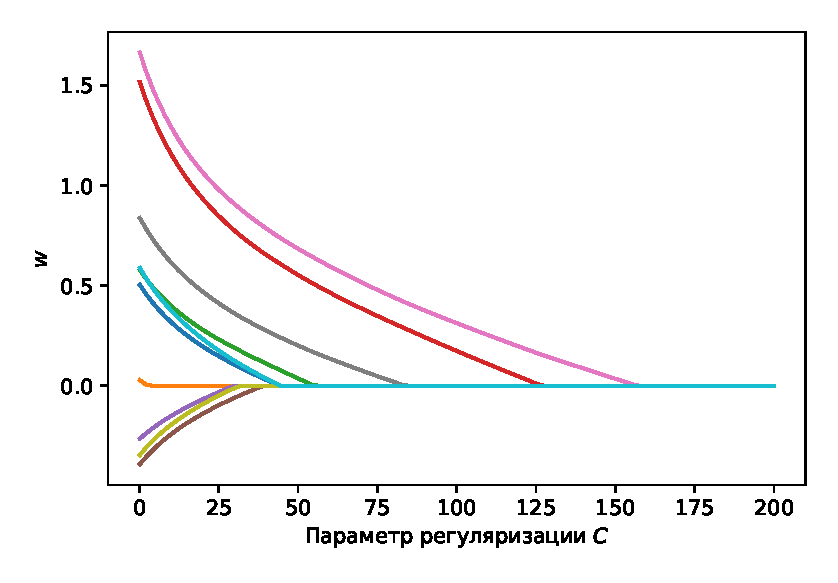
\includegraphics[width=0.5\textwidth]{../figures/log_reg_cs_exp.eps}
	\caption{Sample figure caption.}
	\label{fig:fig1}
\end{figure}

\subsection{Tables}
See awesome Table~\ref{tab:table}.

The documentation for \verb+booktabs+ (`Publication quality tables in LaTeX') is available from:
\begin{center}
	\url{https://www.ctan.org/pkg/booktabs}
\end{center}


\begin{table}
	\caption{Sample table title}
	\centering
	\begin{tabular}{lll}
		\toprule
		\multicolumn{2}{c}{Part}                   \\
		\cmidrule(r){1-2}
		Name     & Description     & Size ($\mu$m) \\
		\midrule
		Dendrite & Input terminal  & $\sim$100     \\
		Axon     & Output terminal & $\sim$10      \\
		Soma     & Cell body       & up to $10^6$  \\
		\bottomrule
	\end{tabular}
	\label{tab:table}
\end{table}

\subsection{Lists}
\begin{itemize}
	\item Lorem ipsum dolor sit amet
	\item consectetur adipiscing elit.
	\item Aliquam dignissim blandit est, in dictum tortor gravida eget. In ac rutrum magna.
\end{itemize}


\bibliographystyle{unsrtnat}
\bibliography{references}

\end{document}